\documentclass[11pt,a4paper,]{article}
\usepackage{lmodern}
\usepackage{amssymb,amsmath}
\usepackage{ifxetex,ifluatex}
\usepackage{fixltx2e} % provides \textsubscript
\ifnum 0\ifxetex 1\fi\ifluatex 1\fi=0 % if pdftex
  \usepackage[T1]{fontenc}
  \usepackage[utf8]{inputenc}
\else % if luatex or xelatex
  \ifxetex
    \usepackage{mathspec}
  \else
    \usepackage{fontspec}
  \fi
  \defaultfontfeatures{Ligatures=TeX,Scale=MatchLowercase}
\fi
% use upquote if available, for straight quotes in verbatim environments
\IfFileExists{upquote.sty}{\usepackage{upquote}}{}
% use microtype if available
\IfFileExists{microtype.sty}{%
\usepackage{microtype}
\UseMicrotypeSet[protrusion]{basicmath} % disable protrusion for tt fonts
}{}
\usepackage[margin=1in]{geometry}
\usepackage{hyperref}
\hypersetup{unicode=true,
            pdftitle={Diagnosing outliers and visualization of quantile regression models},
            pdfauthor={Wenjing Wang1, Dianne Cook2, Earo Wang2; 1Renmin University of China , 2Monash University},
            pdfborder={0 0 0},
            breaklinks=true}
\urlstyle{same}  % don't use monospace font for urls
\usepackage{color}
\usepackage{fancyvrb}
\newcommand{\VerbBar}{|}
\newcommand{\VERB}{\Verb[commandchars=\\\{\}]}
\DefineVerbatimEnvironment{Highlighting}{Verbatim}{commandchars=\\\{\}}
% Add ',fontsize=\small' for more characters per line
\usepackage{framed}
\definecolor{shadecolor}{RGB}{248,248,248}
\newenvironment{Shaded}{\begin{snugshade}}{\end{snugshade}}
\newcommand{\KeywordTok}[1]{\textcolor[rgb]{0.13,0.29,0.53}{\textbf{{#1}}}}
\newcommand{\DataTypeTok}[1]{\textcolor[rgb]{0.13,0.29,0.53}{{#1}}}
\newcommand{\DecValTok}[1]{\textcolor[rgb]{0.00,0.00,0.81}{{#1}}}
\newcommand{\BaseNTok}[1]{\textcolor[rgb]{0.00,0.00,0.81}{{#1}}}
\newcommand{\FloatTok}[1]{\textcolor[rgb]{0.00,0.00,0.81}{{#1}}}
\newcommand{\ConstantTok}[1]{\textcolor[rgb]{0.00,0.00,0.00}{{#1}}}
\newcommand{\CharTok}[1]{\textcolor[rgb]{0.31,0.60,0.02}{{#1}}}
\newcommand{\SpecialCharTok}[1]{\textcolor[rgb]{0.00,0.00,0.00}{{#1}}}
\newcommand{\StringTok}[1]{\textcolor[rgb]{0.31,0.60,0.02}{{#1}}}
\newcommand{\VerbatimStringTok}[1]{\textcolor[rgb]{0.31,0.60,0.02}{{#1}}}
\newcommand{\SpecialStringTok}[1]{\textcolor[rgb]{0.31,0.60,0.02}{{#1}}}
\newcommand{\ImportTok}[1]{{#1}}
\newcommand{\CommentTok}[1]{\textcolor[rgb]{0.56,0.35,0.01}{\textit{{#1}}}}
\newcommand{\DocumentationTok}[1]{\textcolor[rgb]{0.56,0.35,0.01}{\textbf{\textit{{#1}}}}}
\newcommand{\AnnotationTok}[1]{\textcolor[rgb]{0.56,0.35,0.01}{\textbf{\textit{{#1}}}}}
\newcommand{\CommentVarTok}[1]{\textcolor[rgb]{0.56,0.35,0.01}{\textbf{\textit{{#1}}}}}
\newcommand{\OtherTok}[1]{\textcolor[rgb]{0.56,0.35,0.01}{{#1}}}
\newcommand{\FunctionTok}[1]{\textcolor[rgb]{0.00,0.00,0.00}{{#1}}}
\newcommand{\VariableTok}[1]{\textcolor[rgb]{0.00,0.00,0.00}{{#1}}}
\newcommand{\ControlFlowTok}[1]{\textcolor[rgb]{0.13,0.29,0.53}{\textbf{{#1}}}}
\newcommand{\OperatorTok}[1]{\textcolor[rgb]{0.81,0.36,0.00}{\textbf{{#1}}}}
\newcommand{\BuiltInTok}[1]{{#1}}
\newcommand{\ExtensionTok}[1]{{#1}}
\newcommand{\PreprocessorTok}[1]{\textcolor[rgb]{0.56,0.35,0.01}{\textit{{#1}}}}
\newcommand{\AttributeTok}[1]{\textcolor[rgb]{0.77,0.63,0.00}{{#1}}}
\newcommand{\RegionMarkerTok}[1]{{#1}}
\newcommand{\InformationTok}[1]{\textcolor[rgb]{0.56,0.35,0.01}{\textbf{\textit{{#1}}}}}
\newcommand{\WarningTok}[1]{\textcolor[rgb]{0.56,0.35,0.01}{\textbf{\textit{{#1}}}}}
\newcommand{\AlertTok}[1]{\textcolor[rgb]{0.94,0.16,0.16}{{#1}}}
\newcommand{\ErrorTok}[1]{\textcolor[rgb]{0.64,0.00,0.00}{\textbf{{#1}}}}
\newcommand{\NormalTok}[1]{{#1}}
\usepackage{longtable,booktabs}
\usepackage{graphicx,grffile}
\makeatletter
\def\maxwidth{\ifdim\Gin@nat@width>\linewidth\linewidth\else\Gin@nat@width\fi}
\def\maxheight{\ifdim\Gin@nat@height>\textheight\textheight\else\Gin@nat@height\fi}
\makeatother
% Scale images if necessary, so that they will not overflow the page
% margins by default, and it is still possible to overwrite the defaults
% using explicit options in \includegraphics[width, height, ...]{}
\setkeys{Gin}{width=\maxwidth,height=\maxheight,keepaspectratio}
\IfFileExists{parskip.sty}{%
\usepackage{parskip}
}{% else
\setlength{\parindent}{0pt}
\setlength{\parskip}{6pt plus 2pt minus 1pt}
}
\setlength{\emergencystretch}{3em}  % prevent overfull lines
\providecommand{\tightlist}{%
  \setlength{\itemsep}{0pt}\setlength{\parskip}{0pt}}
\setcounter{secnumdepth}{5}
% Redefines (sub)paragraphs to behave more like sections
\ifx\paragraph\undefined\else
\let\oldparagraph\paragraph
\renewcommand{\paragraph}[1]{\oldparagraph{#1}\mbox{}}
\fi
\ifx\subparagraph\undefined\else
\let\oldsubparagraph\subparagraph
\renewcommand{\subparagraph}[1]{\oldsubparagraph{#1}\mbox{}}
\fi

%%% Use protect on footnotes to avoid problems with footnotes in titles
\let\rmarkdownfootnote\footnote%
\def\footnote{\protect\rmarkdownfootnote}

%%% Change title format to be more compact
\usepackage{titling}

% Create subtitle command for use in maketitle
\newcommand{\subtitle}[1]{
  \posttitle{
    \begin{center}\large#1\end{center}
    }
}

\setlength{\droptitle}{-2em}
  \title{Diagnosing outliers and visualization of quantile regression models}
  \pretitle{\vspace{\droptitle}\centering\huge}
  \posttitle{\par}
  \author{Wenjing Wang\textsuperscript{1}, Dianne Cook\textsuperscript{2}, Earo
Wang\textsuperscript{2} \\ \textsuperscript{1}Renmin University of China ,
\textsuperscript{2}Monash University}
  \preauthor{\centering\large\emph}
  \postauthor{\par}
  \date{}
  \predate{}\postdate{}


\usepackage{amsthm}
\newtheorem{theorem}{Theorem}[section]
\newtheorem{lemma}{Lemma}[section]
\theoremstyle{definition}
\newtheorem{definition}{Definition}[section]
\newtheorem{corollary}{Corollary}[section]
\newtheorem{proposition}{Proposition}[section]
\theoremstyle{definition}
\newtheorem{example}{Example}[section]
\theoremstyle{remark}
\newtheorem*{remark}{Remark}
\begin{document}
\maketitle

{
\setcounter{tocdepth}{2}
\tableofcontents
}
\section{Introduction}\label{introduction}

\subsection{Background of quantile
regression}\label{background-of-quantile-regression}

Quantile regression model has been widely used in many research areas
such as economy, finance, social science and many other areas (Autor,
Houseman and Kerr (2017), Mitchell, Dowda and Pate (2017),
Gallego-Álvarez and Ortas (2017), Korobilis (2017), Maciejowska,
Nowotarski and Weron (2016)). Observed covariates in quantile regression
can describe the distribution of response variable which extend the mean
regression analysis. In addition, mean regression can no longer maintain
the optimal properties due to heteroscedasticity or heavy tail
distribution.

Linear quantile regression model can be present as
\(y=X^{'}\beta+\epsilon\), where \(y\) is response variable, \(X\) is
covariate variable vector, \(\beta\) and \(\epsilon\) are coefficient
vector and error term. The \(\tau\)th quantile function of the sample is
\(Q_{y}(\tau|x)=X^{'}\beta(\tau)\). Based on the idea of minimizing a
sum of asymmetrically weighted absolute residuals, the objective
function of quantile regression model is,

\[\min\sum_{i=1}^{n} \rho_{\tau}(y_i-X^{'}\beta)\]

where \(\rho(.)\) is loss function which was defined as
\(\rho_{\tau}(u)=u(\tau-I(u <0))\)

Assuming \(Y_1,...,Y_n\) is a sequence of i.i.d random variables, which
has distribution function \(F\) and continuous density function \(f\).
The covariant matrix is \(\textbf{X}\). Quantile regressoin coefficient
vector \(\hat{\beta}_{\tau}\) is asymptotically normal,

\[\sqrt{n}(\hat{\beta}_{\tau}-\beta_{\tau}) \xrightarrow{d} N(0, \tau(1-\tau)D^{-1}\varOmega_{x}D^{-1})\]

where

\(D=E(f(\textbf{X}\beta)\textbf{XX^{'}})\) and
\(\varOmega_{x}=E(\textbf{X}^{'}\textbf{X})\)

In current research trend, quantile regression has been embeded in other
models to enhance model features or conduct better results analysis.
Geraci (2014) proposed linear quantile mixed model which dealt with
within-subject dependence by embeding subject-specific random intercepts
into quantile regression model. Chernozhukov and Hansen (2006) used
instrumental variable quantile regression for heterogeneous treatment
effect models and simulaneous equations models to evaluate the impact of
endogenous variables or treatments on the entire distribution of
outcomes.

Another development is fitting quantile regression for specified data
class. Koenker (2004), Geraci and Bottai (2006) proposed to conduct
quantile regression for longitudinal data. Parente and Santos Silva
(2016) studied properties of the quantile regression estimator when data
are sampled from independent and identically distributed clusters. Canay
(2011), Arellano and Bonhomme (2016) introduce a class of quantile
regression estimators for short panels. Galvao and Kato (2016),
presented fixed effects estimation of quantile regression models for
panel data.

Extensive theories has been used for inferencing quantile regression
parameters. Gutenbrunner, Jureckova, Koenker, and Portnoy (1993)
proposed rank-based inference to deal problems of constructing
confidence intervals for individual quantile regression parameter
estimates. Hahn (1995), Horowitz (1998), Fitzenberger (1998), He and Hu
(1999) contributed to a variety of resampling methods to quantifying the
robustness of inferencing. Koneker and Machado (1999) discussed
inference for quantile regression based on Kolmogorov-Smironov goodness
of fit method. To deal with ``the Durbin problem'', Koenker and Xiao
(2002) developed new tests of the location shift and location-scale
shift models for quantile regression process. There are also studies of
quantile regression in bayesian framework which extended research ideas.

Based on above numerous of methodology and application studies of
quantile regression, extensive toolboxs conduct model fitting and
inference has been developed. Free software R offers several packages
implementing quantile regression, most famous \texttt{quantreg} by Roger
Koenker, but also \texttt{gbm}, \texttt{quantregForest}, \texttt{qrnn},
\texttt{ALDqr} and \texttt{bayesQR}. However, few model diagnostic
methods were proposed for quantile regression and no toolbox for model
diagnostic were implemented in R. Statistical software SAS offered
simple outlier diagnostic methods in procedure \texttt{QUANTREG}.
Koenker(2017) also pointed out that more work needs to be done to
develop better diagnostic tools for quantile regression models.

\subsection{Outlier detection in regression and
HLMdiag}\label{outlier-detection-in-regression-and-hlmdiag}

Sample data from the real world may have special points located far away
from others. In regression model, these points may affect model fitting.
In single variabe case, we can observe outliers based on scatter plot.
Difficulty lies in high-dimensional situation, where statistical methods
should be used.

Outliers in regression can be divided into two class, one is outliers in
vertical direction and the other is leverage point. Various methods for
detecting outliers have been studied(Atkinson 1994; Barnett and Lewis
1994; Becker and Gather 1999, 2001; Davies and Gather 1993; Gather and
Becker 1997; Gnanadesikan and Kettenking 1972; Hadi 1992, 1994; Hawkins
1980; Maronna and Yohai 1995; Penny 1995; Rocke and Woodruff 1996;
Rousseeuw and Van Zomeren 1990). Commonly used methods in mean
regression including residuals, leverage value, studentized residuals
and jacknife residuals.

Classic least ordinary square estimation of linear regresssion can be
expressed as \(\hat{\beta}=(X^{'}X)^{-1}X^{'}Y\),
\(\hat{Y}=X(X^{'}X)^{-1}X^{'}Y=HY\), where, \(H\) is called hat matrix.
Residuals can be write as
\(\hat{\epsilon}=Y-\hat{Y}(1-H)Y=(1-H)\epsilon\). The variance of the
error term and the estimation of \(Y\) are
\(Var(\hat{\epsilon})=(1-H)\),
\(Var(\hat{Y})=X\hat{\beta}=H\sigma^{2}\).

If taking outliers in \(y\) and leverage points all in consideration, we
can construct studentized residuals, which is
\(r_i=\frac{\hat{\epsilon}_{i}}{\sigma^{2}\sqrt{1-h_i}}\). The larger
\(r_i\), the more suspicious the outlier is.Another widely used outlier
diagnositc idea is \texttt{leave-one-out}. Jackknif residual, knowing as
\(t_i=\frac{\hat{y}_{(i)}-\hat{y_i}}{\hat{\sigma}_{(i)}(1+x^{'}_{i}(X^{'}_{(i)}X_{(i)})^{-1}x_{i})^{-1/2}}\)
and cook distance used this idea.

\section{Outlier detection in quantile
regression}\label{outlier-detection-in-quantile-regression}

Due to the robust property of quantiles, quantile regressions are
relatively robust towards outliers than mean regression model, This
property has been discussed by Onyedikachi(2015). They used influence
funtion to discuss the property of robustness of quantile regression.

Suppose \(T\) is a function of \(F\), the influence function is the
directional derivative of \(T(F)\) at \(F\), and it measures the effect
of a small perturbation in \(F\) on \(T(F)\). For the \(\tau\)th
quantile points, influence function can be expressed as,

\begin{equation}

IF(y;T;F)=\left\{
\begin{aligned}
\frac{\tau}{f(F^{-1}(\tau))} & ; & y > F^{-1}(\tau) \\
\frac{(\tau-1)}{f(F^{-1}(\tau))} & ; & y \leq F^{-1}(\tau) 
\end{aligned}
\right.

(\#eq:quantile_influence)
\end{equation}

The influence function @ref(eq:quantile\_influence) indicate that the
contamination in \(y\) on quantile points is bounded. Onyedikachi(2015)
also provided the influence function for quantile regression.

Let \(F\) represent the joint distribution of the pairs \((x,y)\), we
have,

\begin{equation}
IF((y,x),\hat{\beta}_{F(\tau)},F)=Q^{-1}xsgn(y-x^{'}\hat{\beta}_{F}(\tau))
(\#eq:quantile_regression_influence)
\end{equation}

where

\begin{equation}
dF=dG(x)f(y|x)dy
(\#eq: dg)
\end{equation}

\begin{equation}
Q=\int xx^{'}f(X^{'}\hat{\beta}_{F}(\tau))dG(x)
(\#eq: q_influence)
\end{equation}

@ref(eq:quantile\_regression\_influence) implies that in quantile
regression, the quantile regression estimates will not be affected by
any chagne in the value of the dependent variable for some observations
as long as the relative positions of the observation points to the
fitted plane are maintained.

\subsection{Displaying how do the outliers affect quantile
regression}\label{displaying-how-do-the-outliers-affect-quantile-regression}

We conducted simulation to display how does outliers affect quantile
regression estimations. In two simple simulation studies, we generate
100 sample observation and 3 outliers. The outliers are distributed in
two locations in each case. We fitted mean regression and quantile
regression based on these dataset to observe how do outliers affect
model coefficients.

\begin{figure}

{\centering \includegraphics{Diagnosing_outliers_and_visualization_of_quantile_regression_models_files/figure-latex/unnamed-chunk-2-1} 

}

\caption{Fitting quantile regression model on quantile 0.1, 0.5 and 0.9 using simulated datasets with and without outliers. The outliers located at the top-left of the original dataset. Results show that outliers pull up the slope of the 0.9 and 0.1 regression line. When outliers located at the bottom-right of the original dataset, results show that outliers pull down the slope of the 0.1 regression line.}\label{fig:unnamed-chunk-2}
\end{figure}

We also change the location of outliers or add outliers numbers to
observe how they affect coeficient estimations on each quantile. These
simulation studies are extended to multi-variables model.Using the
simulated data to construct quantile regression model. By comparing the
four models, we have a brief idea of the effect of outliers locating.
The results show that when outliers moving down in y direction for 10
unit, it pulls down the slope on every quantile(comparing the result of
model rq(y1\textasciitilde{}x) and rq(y2\textasciitilde{}x)). However,
keeping moving down the outliers does no change to the slopes. This
reflect the boundary theory expressed by influence function above.

\begin{figure}

{\centering 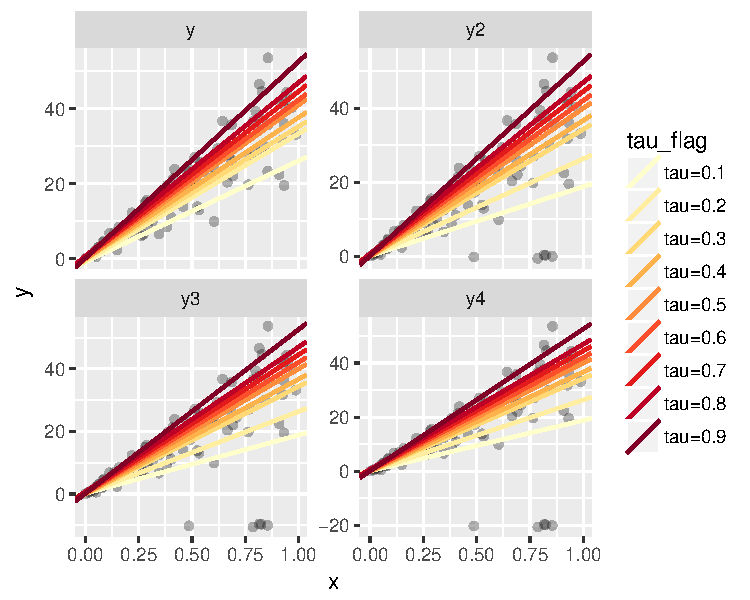
\includegraphics{Diagnosing_outliers_and_visualization_of_quantile_regression_models_files/figure-latex/move-y1-1} 

}

\caption{Left fig: Fitting quantile regression models using simulated data. We keep moving down the outliers in y direction in y2 (y-5), y3 (y-10) and y4 (y-15). Right fig: Fitting quantile regression models using simulated data. We keep moving down the outliers in y direction getting datasets with variable y2 (=y-5), y3 (=y-10) and y4 (=y-15). Results show that in single predictor case, outliers moving down in y make no difference to the quantile regression coefficients estimations}\label{fig:move-y1}
\end{figure}

We also observed the change of coefficients in multi-variable model. The
results show that coefficients changes slowly when keep moving down the
outliers in y-direction.

\begin{figure}

{\centering 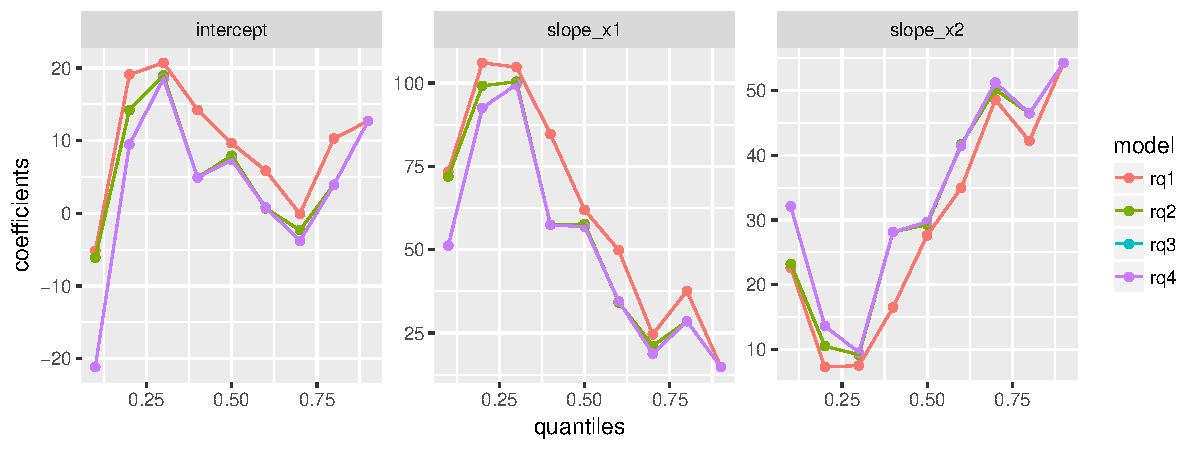
\includegraphics{Diagnosing_outliers_and_visualization_of_quantile_regression_models_files/figure-latex/move-y-multi1-1} 

}

\caption{Fitting quantile regression models using simulated data. We keep moving down the outliers in y direction getting three datasets with different locations of outliers (changing in y-aixs, y2 (=y-5), y3 (=y-10) and y4 (=y-15)). Results show that in multi predictors case, outliers moving down in y make small change to the quantile regression coefficients estimations}\label{fig:move-y-multi1}
\end{figure}

If moving outliers in same pattern moving on x direction, slopes change
every time outlier moves. To go further, each move does different effect
on different quantiles.

\begin{figure}

{\centering 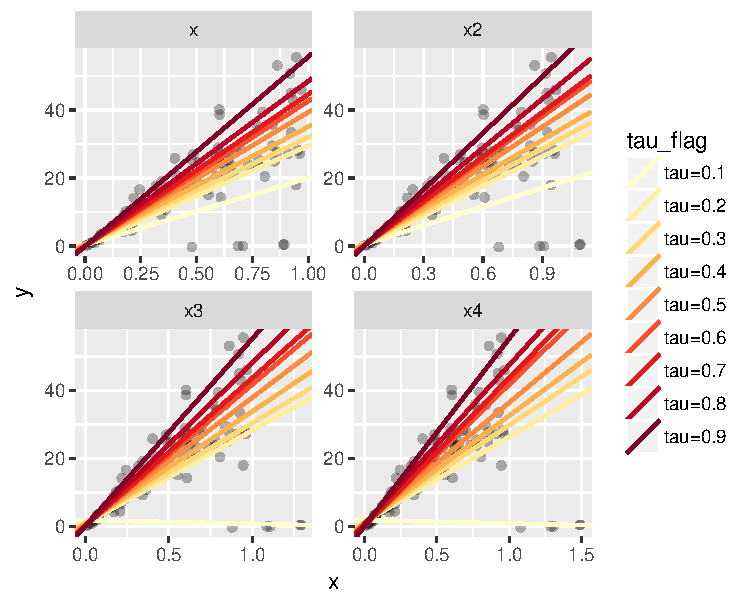
\includegraphics{Diagnosing_outliers_and_visualization_of_quantile_regression_models_files/figure-latex/move-x1-1} 

}

\caption{Left fig: Fitting quantile regression models using simulated data. We keep moving the outliers to the right in x direction getting three datasets with different locations of outliers (changing in x-aixs, x2 (=x+0.2), x3 (=x+0.4) and x4 (=x+0.6)). Right fig: Fitting quantile regression models using simulated data. We keep moving the outliers to the right in x direction getting three datasets with different locations of outliers (changing in x-aixs, x2 (=x+0.2), x3 (=x+0.4) and x4 (=x+0.6)).Results show that in single predictors case, outliers moving right in x make significant change to the quantile regression coefficients estimations.}\label{fig:move-x1}
\end{figure}

In conclusion, quantile regression response differently to outliers
comparing mean regression in two aspects: (a) not all models on each
quantile will be affected when outliers exist. If we are interested in
model on particular quantile, the effect of outliers should be carefully
considered. (b) quantile regression model do not have robustness
properties to so called leverage points.

\section{Outlier diagnosting methods for quantile
regression}\label{outlier-diagnosting-methods-for-quantile-regression}

We proposed three methods for quantile regression outlier diagnostic
which will be discussed as follows.

\begin{itemize}
\tightlist
\item
  Standard residual-Robust Distance
\end{itemize}

Leverage points can not be detected using the famous ``Hat Matrix'' in
quantile regression since the coefficient estimation of quantile
regression do not satisfy \(\hat{\beta}=(X^{'}X)^{-1}X^{'}Y\). One way
to identify possible multivariate outliers is to calculate a distance
from each point to a ``center'' of the data. An outlier would then be a
point with a distance larger than some predetermined cutoff. A
conventional measurement of quadradic distance from a point \(X\) to a
location \(Y\) given given a shape \(S\), in the multivariate setting
is:

\[d^{2}_{S}(X,Y)=(X-Y)^{'}S^{-1}(X-Y)\]

This distance is often called Mahalanobis squared distance(MSD). If
there are only a few outliers, large values of
\(d^{2}_{S}(x_i, \bar{X})\), when \(\bar{X}\) and \(S\) are the standard
sample mean and covariance matrix, indicate that the point \(x_i\) is an
outlier(Barnett and Lewis 1994). The distribution of the MSD with both
the true location and shape parameters and the standard sample location
and shape parameters is well known(Gnanadesikan and Kettenring 1972).
However, the standard sample locatoin and shape parameters are not
robust to outliers, and the distributional fit to the distance breaks
down when robust measures of location and shape are used in the
MSD(Rousseeuw and van Zomeren 1991). Datasets with multiple outliers or
clusters of outliers are subject to problems of masking and
swamping(Pearson and Chandra Sekar 1936).

Problems of masking and swamping can be resolved by using robust
estimates of shape and location, which by definition are less affected
by outliers. We use Rousseeuw's minimum covariance
determinant(MCD)(Rousseeuw 1985) to estimate the location and shape of
the data.

The MCD estimator is a robust, high-breakdown point which can be defined
as:

\[MCD = (\bar{X}^{*}_{h}, S^{*}_{h})\] where
\(h={p: |S^{*}_{h}|<|S^{*}_{k}|,|k|=p}\),
\(\bar{X}^{*}_{h}=\frac{1}{p}\sum_{i \in p}x_{i}\),
\(S^{*}_{p}=\frac{1}{p}\sum_{i \in p}(x_i-\bar{X}^{*}_{p})(x_i-\bar{X}^{*}_{p})^{'}\).

The value \(p\) can be thought of as the minimum number of points which
must not be outliers. The MCD has its highest possible breakdown at
\(h=[\frac{n+p+1}{2}]\) where \([.]\) is the greatest integer function.
Because we are interested in outlier detection, we will use \(h\) at its
highest possible breakdown. \(h=[\frac{n+p+1}{2}]\) in our calculations,
and we refer to a sample of size \(h\) as a ``half sample'' The MCD is
omputed from the ``closet'' half sample, and therefore, the outlying
points will have little affect on the MCD location or shape estimate.

We use MCD to detect outliers in covariates and use absolute standard
residuals to detect outliers in y direction.

\begin{itemize}
\tightlist
\item
  Generalized Cook Distance
\end{itemize}

To assess the influence of the \(i\)th case on the coefficient
estimation of quantile regression, we compare the difference between
\(\hat{\theta}_{[i]}\) and \(\hat{\theta}\).

Case-deletion is a classical approach to study the effects of dropping
the \(i\)th observation deleted. Thus, the complete-data log-likelihood
function based on the data with the \(i\)th case deleted will be denoted
by \(L_{c}(\theta|y_{c[i]})\). Let
\(\hat{\theta}_{[i]}=(\hat{\beta}^{T}_{p[i]}, \hat{\sigma}^{2}_{[i]})^{T}\)
be the maximizer of the function
\(Q_{[i]}(\theta|\hat{\theta})=E_{\hat{\theta}}[l_{c}(\theta|Y_{c[i]})|y]\),
where \(\hat{\theta}=(\hat{\beta}^{T}, \hat{\sigma}^{2})^{T}\) is the ML
estimate of \(\theta\).

To calculate the case-deletion estimate \(\hat{\theta}_{[i]}\) of
\(\theta\), proposed the following one-step approximation based on
Q-function,

\[\hat{\theta}_{[i]}=\hat{\theta}+\{-Q(\hat{\theta}|\hat{\theta})\}^{-1}Q_{[i]}(\hat{\theta}|\hat{\theta})\]

where

\[Q(\hat{\theta}|\hat{\theta})=\frac{\partial^{2}Q(\theta|\hat{\theta})}{\partial\theta\partial \theta^{T}}|_{\theta=\hat{\theta}}\]

\[Q_{[i]}(\hat{\theta}|\hat{\theta})=\frac{\partial Q_{[i]}(\theta|\hat{\theta})}{\partial\theta}|_{\theta=\hat{\theta}}\]

are the Hessian matrix and the gradient vector evaluated at
\(\hat{\theta}\), respectively.

For measuring the distance between \(\hat{\theta}_{[i]}\) and
\(\hat{\theta}\). We consider generalized cook distance as follows.

\[GD_{i} =(\hat{\theta}_{[i]}-\hat{\theta})^{T}\{-Q(\hat{\theta}|\hat{\theta})\}(\hat{\theta}_{[i]}-\hat{\theta}), i=1,...,n\]

\begin{itemize}
\tightlist
\item
  Q-function Distance
\end{itemize}

The measurement of the influence of the \(i\)th case is based on the
Q-distance function, similar to the likelihood distance \(LD_{i}\) which
was defined as

\[QD_{i}=2\{Q(\hat{\theta}|\hat{\theta})-Q(\hat{\theta}_{[i]}|\hat{\theta})\}\]

\begin{itemize}
\tightlist
\item
  Mean Post Probability
\end{itemize}

Baysian quantile regression added a latent variable \(v_i\) into model
for each observation. Every \(v_i\) is assumed to have an exponential
distribution with mean \(\sigma\), that with the likelihood produces a
posterior distributed according to a generalized inverse Gaussian with
parameters.

If we define the variable \(O_i\), which takes value equal to 1 when the
\(i\)th observation is an outlier, and 0 otherwise. Then we propose to
calculate the pro bility of an observation being an outlier as

\[P(O_i=1)=\frac{1}{n-1}\sum_{j \neq i}P(v_i > v_j|data)\]

The probability in the expression above can be approximated given the
MCMC draws, as follows:

\[P(O_i = 1)=\frac{1}{M}I(v^{(l)_i}>max_{k \in 1:M}v^{(k)}_j)\]

where \(M\) is the size of the chain of \(v_i\) after the burn-in perior
and \(v^{(l)}_i\) is the \(l\)th draw of this chain.

\begin{itemize}
\tightlist
\item
  K-L Divergence
\end{itemize}

Similar with mean posterior probability method, we also caculates
Kullback-Leibler divergence which proposed by Kullback and Leibler(1951)
as a more precise method of measuring the distance between those latent
variables in Bayes quantile regression. The Kullback-Leibler divergence
is defined as:

\[K(f_i, f_j)=\int log(\frac{f_i(x)}{f_j(x)}f_{i}(x))dx\]

where \(f_i\) could be the posterior conditional distribution of \(v_i\)
and \(f_j\) the posterior conditional distribution of \(v_j\). We should
average this divergence for one observation based on the distance from
all others,

\[KL(f_i)=\frac{1}{n-1}\sum_{j\neq i}K(f_i, f_j)\]

The outliers should show a high probability value for this divergence.
We compute the integral using the trapezoidal rule.

\section{Examining outlier detection}\label{examining-outlier-detection}

We developed R package \texttt{quokar} to implete quantile regression
outlier diagnostic methods. This package mainly realized two basic
features: (a) plot the outlier states; (b) plot data with outliers
marked. \texttt{quokar} is available from Github at
\url{https://github.com/wenjingwang/quokar}, so to install and load
withn R use:

\begin{Shaded}
\begin{Highlighting}[]
\NormalTok{devtools::}\KeywordTok{install_github}\NormalTok{(}\StringTok{"wenjingwang/quokar"}\NormalTok{)}
\end{Highlighting}
\end{Shaded}

\begin{verbatim}
## Skipping install of 'quokar' from a github remote, the SHA1 (a67b8ff7) has not changed since last install.
##   Use `force = TRUE` to force installation
\end{verbatim}

\begin{Shaded}
\begin{Highlighting}[]
\KeywordTok{library}\NormalTok{(quokar)}
\end{Highlighting}
\end{Shaded}

We implete ais data as an example to introduce this package. AIS data
include 14 variables for 100 female atheletes.

\subsection{Plot the outlier stats}\label{plot-the-outlier-stats}

In single variable case, we can use scatter plot to represent the
outlier stats. The following code showed how to display suspicious
outliers based on quantile regression models.

\begin{Shaded}
\begin{Highlighting}[]
\KeywordTok{data}\NormalTok{(ais)}
\NormalTok{ais_female <-}\StringTok{ }\KeywordTok{filter}\NormalTok{(ais, Sex ==}\StringTok{ }\DecValTok{1}\NormalTok{)}
\NormalTok{case <-}\StringTok{ }\DecValTok{1} \NormalTok{:}\StringTok{ }\KeywordTok{nrow}\NormalTok{(ais_female)}
\NormalTok{ais_female <-}\StringTok{ }\KeywordTok{cbind}\NormalTok{(case, ais_female)}
\NormalTok{coef_rq <-}\StringTok{ }\KeywordTok{coef}\NormalTok{(}\KeywordTok{rq}\NormalTok{(BMI ~}\StringTok{ }\NormalTok{LBM, }\DataTypeTok{tau =} \KeywordTok{c}\NormalTok{(}\FloatTok{0.1}\NormalTok{, }\FloatTok{0.5}\NormalTok{, }\FloatTok{0.9}\NormalTok{),}
                   \DataTypeTok{data =} \NormalTok{ais_female, }\DataTypeTok{method =} \StringTok{"br"}\NormalTok{))}

\NormalTok{br_coef <-}\StringTok{ }\KeywordTok{data.frame}\NormalTok{(}\DataTypeTok{intercept =} \NormalTok{coef_rq[}\DecValTok{1}\NormalTok{, ],}
                      \DataTypeTok{coef =} \NormalTok{coef_rq[}\DecValTok{2}\NormalTok{, ],}
                      \DataTypeTok{tau_flag =} \KeywordTok{colnames}\NormalTok{(coef_rq))}
\KeywordTok{ggplot}\NormalTok{(ais_female)+}
\StringTok{  }\KeywordTok{geom_point}\NormalTok{(}\KeywordTok{aes}\NormalTok{(}\DataTypeTok{x =} \NormalTok{LBM, }\DataTypeTok{y =} \NormalTok{BMI)) +}
\StringTok{  }\KeywordTok{geom_abline}\NormalTok{(}\DataTypeTok{data =} \NormalTok{br_coef, }\KeywordTok{aes}\NormalTok{(}\DataTypeTok{intercept =} \NormalTok{intercept,}
                                  \DataTypeTok{slope =} \NormalTok{coef,}
                                  \DataTypeTok{colour =} \NormalTok{tau_flag), }\DataTypeTok{size =} \DecValTok{1}\NormalTok{) +}
\StringTok{  }\KeywordTok{geom_text}\NormalTok{(}\DataTypeTok{data =} \KeywordTok{subset}\NormalTok{(ais_female, case %in%}\StringTok{ }\KeywordTok{c}\NormalTok{(}\DecValTok{1}\NormalTok{, }\DecValTok{75}\NormalTok{)),}
                          \KeywordTok{aes}\NormalTok{(}\DataTypeTok{x =} \NormalTok{LBM, }\DataTypeTok{y =} \NormalTok{BMI, }\DataTypeTok{label =} \NormalTok{case), }
            \DataTypeTok{colour =} \StringTok{"red"}\NormalTok{,}\DataTypeTok{hjust =} \DecValTok{0}\NormalTok{, }\DataTypeTok{vjust =} \DecValTok{0}\NormalTok{) +}
\StringTok{  }\KeywordTok{scale_colour_brewer}\NormalTok{(}\StringTok{"Dark2"}\NormalTok{) +}
\StringTok{  }\KeywordTok{theme_dark}\NormalTok{()}
\end{Highlighting}
\end{Shaded}

\begin{figure}

{\centering 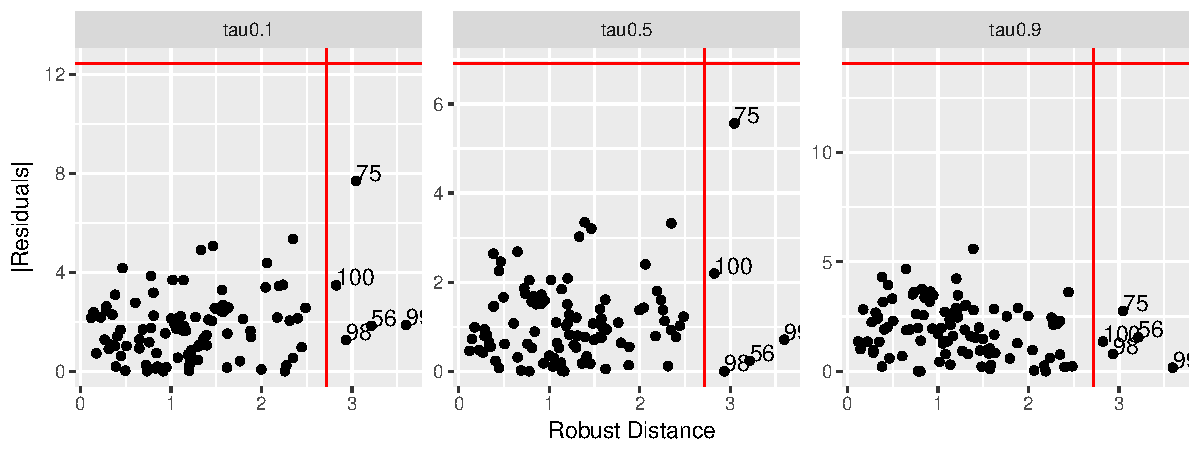
\includegraphics{Diagnosing_outliers_and_visualization_of_quantile_regression_models_files/figure-latex/unnamed-chunk-4-1} 

}

\caption{Plot the outlier stats.}\label{fig:unnamed-chunk-4}
\end{figure}

\subsection{Plot data with outliers
marked}\label{plot-data-with-outliers-marked}

Scatter plot has limitations when tackling multi-variable regression
cases. In \texttt{quokar}, we provide functions to do outlier diagnostic
which return the dataframe easily to plot data with outliers marked.

\begin{itemize}
\tightlist
\item
  residual-robust distance method
\end{itemize}

First, we calculate residuals, mahananobi distance and robust distance
for quantile regression using function \texttt{plot\_distance}.
Simutaneously, it provides the cutoff value for identifying the outliers
in regression models.

\begin{Shaded}
\begin{Highlighting}[]
\NormalTok{tau <-}\StringTok{ }\KeywordTok{c}\NormalTok{(}\FloatTok{0.1}\NormalTok{, }\FloatTok{0.5}\NormalTok{, }\FloatTok{0.9}\NormalTok{)}
\NormalTok{object <-}\StringTok{ }\KeywordTok{rq}\NormalTok{(BMI ~}\StringTok{ }\NormalTok{LBM +}\StringTok{ }\NormalTok{Bfat, }\DataTypeTok{data =} \NormalTok{ais_female, }\DataTypeTok{tau =} \NormalTok{tau)}
\NormalTok{plot_distance <-}\StringTok{ }\KeywordTok{frame_distance}\NormalTok{(object, }\DataTypeTok{tau =} \KeywordTok{c}\NormalTok{(}\FloatTok{0.1}\NormalTok{, }\FloatTok{0.5}\NormalTok{, }\FloatTok{0.9}\NormalTok{))}
\NormalTok{distance <-}\StringTok{ }\NormalTok{plot_distance[[}\DecValTok{1}\NormalTok{]]}
\KeywordTok{head}\NormalTok{(distance, }\DecValTok{3}\NormalTok{)}
\end{Highlighting}
\end{Shaded}

\begin{verbatim}
##          md        rd tau_flag  residuals
## 1 1.2275233 1.3912428   tau0.1 -1.4630550
## 2 0.6988854 0.6486756   tau0.1 -0.9262022
## 3 0.3836449 0.3315911   tau0.1  1.0706377
\end{verbatim}

\begin{Shaded}
\begin{Highlighting}[]
\NormalTok{cutoff_v <-}\StringTok{ }\NormalTok{plot_distance[[}\DecValTok{2}\NormalTok{]]; cutoff_v}
\end{Highlighting}
\end{Shaded}

\begin{verbatim}
## [1] 2.716203
\end{verbatim}

\begin{Shaded}
\begin{Highlighting}[]
\NormalTok{cutoff_h <-}\StringTok{ }\NormalTok{plot_distance[[}\DecValTok{3}\NormalTok{]]; cutoff_h}
\end{Highlighting}
\end{Shaded}

\begin{verbatim}
## [1] 12.450378  6.917875 14.073312
\end{verbatim}

Function \texttt{plot\_distance} returns the tidy data form for plotting
data with outliers marked and overlaying the cutoff lines.

\begin{Shaded}
\begin{Highlighting}[]
\NormalTok{n <-}\StringTok{ }\KeywordTok{nrow}\NormalTok{(object$model)}
\NormalTok{case <-}\StringTok{ }\KeywordTok{rep}\NormalTok{(}\DecValTok{1}\NormalTok{:n, }\KeywordTok{length}\NormalTok{(tau))}
\NormalTok{distance <-}\StringTok{ }\KeywordTok{cbind}\NormalTok{(case, distance)}
\NormalTok{distance$residuals <-}\StringTok{ }\KeywordTok{abs}\NormalTok{(distance$residuals)}
\NormalTok{tau_flag <-}\StringTok{ }\KeywordTok{paste}\NormalTok{(}\StringTok{"tau"}\NormalTok{, tau, }\DataTypeTok{sep=}\StringTok{""}\NormalTok{)}
\NormalTok{text_flag <-}\StringTok{ }\DecValTok{1}\NormalTok{:}\KeywordTok{length}\NormalTok{(cutoff_h) %>%}
\StringTok{                            }\KeywordTok{map}\NormalTok{(function(i)\{}
                            \NormalTok{distance %>%}\StringTok{ }
\StringTok{                            }\KeywordTok{filter}\NormalTok{((residuals >}\StringTok{ }\NormalTok{cutoff_h[i] |rd >}\StringTok{ }\NormalTok{cutoff_v)}
                                \NormalTok{&}\StringTok{ }\NormalTok{tau_flag ==}\StringTok{ }\NormalTok{tau_flag[i])\})}
\NormalTok{##need polish}
\NormalTok{text_flag_d <-}\StringTok{ }\KeywordTok{rbind}\NormalTok{(text_flag[[}\DecValTok{1}\NormalTok{]], text_flag[[}\DecValTok{2}\NormalTok{]], text_flag[[}\DecValTok{3}\NormalTok{]])}
\KeywordTok{ggplot}\NormalTok{(distance, }\KeywordTok{aes}\NormalTok{(}\DataTypeTok{x =} \NormalTok{rd, }\DataTypeTok{y =} \NormalTok{residuals)) +}
\StringTok{      }\KeywordTok{geom_point}\NormalTok{() +}
\StringTok{      }\KeywordTok{geom_hline}\NormalTok{(}\DataTypeTok{data =} \KeywordTok{data.frame}\NormalTok{(tau_flag, cutoff_h),   }
                 \KeywordTok{aes}\NormalTok{(}\DataTypeTok{yintercept =} \NormalTok{cutoff_h), }\DataTypeTok{colour =} \StringTok{"red"}\NormalTok{) +}
\StringTok{      }\KeywordTok{geom_vline}\NormalTok{(}\DataTypeTok{xintercept =} \NormalTok{cutoff_v, }\DataTypeTok{colour =} \StringTok{"red"}\NormalTok{) +}
\StringTok{      }\KeywordTok{geom_text}\NormalTok{(}\DataTypeTok{data =} \NormalTok{text_flag_d, }\KeywordTok{aes}\NormalTok{(}\DataTypeTok{label =} \NormalTok{case), }\DataTypeTok{hjust =} \DecValTok{0}\NormalTok{, }\DataTypeTok{vjust =} \DecValTok{0}\NormalTok{) +}
\StringTok{      }\KeywordTok{facet_wrap}\NormalTok{(~}\StringTok{ }\NormalTok{tau_flag, }\DataTypeTok{scales =} \StringTok{'free_y'}\NormalTok{) +}
\StringTok{      }\KeywordTok{xlab}\NormalTok{(}\StringTok{"Robust Distance"}\NormalTok{) +}
\StringTok{      }\KeywordTok{ylab}\NormalTok{(}\StringTok{"|Residuals|"}\NormalTok{)}
\end{Highlighting}
\end{Shaded}

\begin{figure}

{\centering 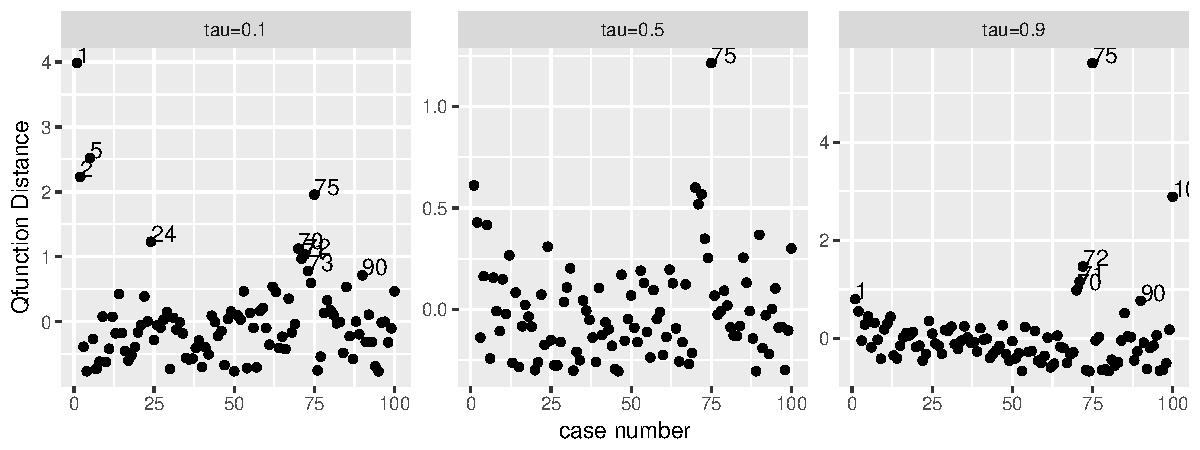
\includegraphics{Diagnosing_outliers_and_visualization_of_quantile_regression_models_files/figure-latex/unnamed-chunk-6-1} 

}

\caption{Robust Distance-Residual Plot. Points on the right of vertical cutoff line are considered leverage points and points above the horizental cutoff line are outliers in y-direction.}\label{fig:unnamed-chunk-6}
\end{figure}

\begin{itemize}
\tightlist
\item
  Generalized cook distance and Q function distance
\end{itemize}

We apply generalized cook distance and Q function distance methods in
function \texttt{frame\_mle}. This function returns generalized cook or
q function distance for regression model on each given quantile. The
results are also in tidy data structure which can be easily used for
plotting the two distances with outliers marked.

\begin{Shaded}
\begin{Highlighting}[]
\NormalTok{y <-}\StringTok{ }\NormalTok{ais_female$BMI}
\NormalTok{x <-}\StringTok{ }\KeywordTok{cbind}\NormalTok{(}\DecValTok{1}\NormalTok{, ais_female$LBM, ais_female$Bfat)}
\NormalTok{case <-}\StringTok{ }\KeywordTok{rep}\NormalTok{(}\DecValTok{1}\NormalTok{:}\KeywordTok{length}\NormalTok{(y), }\KeywordTok{length}\NormalTok{(tau))}
\NormalTok{GCD <-}\StringTok{ }\KeywordTok{frame_mle}\NormalTok{(y, x, tau, }\DataTypeTok{error =} \FloatTok{1e-06}\NormalTok{, }\DataTypeTok{iter =} \DecValTok{10000}\NormalTok{,}
                  \DataTypeTok{method =} \StringTok{'cook.distance'}\NormalTok{)}
\NormalTok{GCD_m <-}\StringTok{ }\KeywordTok{cbind}\NormalTok{(case, GCD)}
\KeywordTok{ggplot}\NormalTok{(GCD_m, }\KeywordTok{aes}\NormalTok{(}\DataTypeTok{x =} \NormalTok{case, }\DataTypeTok{y =} \NormalTok{value )) +}
\StringTok{    }\KeywordTok{geom_point}\NormalTok{() +}
\StringTok{    }\KeywordTok{facet_wrap}\NormalTok{(~variable, }\DataTypeTok{scale =} \StringTok{'free_y'}\NormalTok{) +}
\StringTok{    }\KeywordTok{geom_text}\NormalTok{(}\DataTypeTok{data =} \KeywordTok{subset}\NormalTok{(GCD_m, value >}\StringTok{ }\KeywordTok{mean}\NormalTok{(value) +}\StringTok{ }\DecValTok{2}\NormalTok{*}\KeywordTok{sd}\NormalTok{(value)),}
              \KeywordTok{aes}\NormalTok{(}\DataTypeTok{label =} \NormalTok{case), }\DataTypeTok{hjust =} \DecValTok{0}\NormalTok{, }\DataTypeTok{vjust =} \DecValTok{0}\NormalTok{) +}
\StringTok{    }\KeywordTok{xlab}\NormalTok{(}\StringTok{"case number"}\NormalTok{) +}
\StringTok{    }\KeywordTok{ylab}\NormalTok{(}\StringTok{"Generalized Cook Distance"}\NormalTok{)}
\end{Highlighting}
\end{Shaded}

\begin{figure}

{\centering \includegraphics{Diagnosing_outliers_and_visualization_of_quantile_regression_models_files/figure-latex/unnamed-chunk-7-1} 

}

\caption{Generalized cook distance of each observation on quantile 0.1, 0.5 and 0.9. Case 75 has relative large cook distance-funtion distance to other points}\label{fig:unnamed-chunk-7}
\end{figure}

The same, visualization of Q function diagnostic results are shown in
fig,

\begin{Shaded}
\begin{Highlighting}[]
\NormalTok{QD <-}\StringTok{ }\KeywordTok{frame_mle}\NormalTok{(y, x, tau, }\DataTypeTok{error =} \FloatTok{1e-06}\NormalTok{, }\DataTypeTok{iter =} \DecValTok{10000}\NormalTok{,}
               \DataTypeTok{method =} \StringTok{'qfunction'}\NormalTok{)}
\NormalTok{QD_m <-}\StringTok{ }\KeywordTok{cbind}\NormalTok{(case, QD)}
\KeywordTok{ggplot}\NormalTok{(QD_m, }\KeywordTok{aes}\NormalTok{(}\DataTypeTok{x =} \NormalTok{case, }\DataTypeTok{y =} \NormalTok{value)) +}
\StringTok{ }\KeywordTok{geom_point}\NormalTok{() +}
\StringTok{ }\KeywordTok{facet_wrap}\NormalTok{(~variable, }\DataTypeTok{scale =} \StringTok{'free_y'}\NormalTok{)+}
\StringTok{ }\KeywordTok{geom_text}\NormalTok{(}\DataTypeTok{data =} \KeywordTok{subset}\NormalTok{(QD_m, value >}\StringTok{ }\KeywordTok{mean}\NormalTok{(value) +}\StringTok{ }\KeywordTok{sd}\NormalTok{(value)),}
           \KeywordTok{aes}\NormalTok{(}\DataTypeTok{label =} \NormalTok{case), }\DataTypeTok{hjust =} \DecValTok{0}\NormalTok{, }\DataTypeTok{vjust =} \DecValTok{0}\NormalTok{) +}
\StringTok{ }\KeywordTok{xlab}\NormalTok{(}\StringTok{'case number'}\NormalTok{) +}
\StringTok{ }\KeywordTok{ylab}\NormalTok{(}\StringTok{'Qfunction Distance'}\NormalTok{)}
\end{Highlighting}
\end{Shaded}

\begin{figure}

{\centering \includegraphics{Diagnosing_outliers_and_visualization_of_quantile_regression_models_files/figure-latex/unnamed-chunk-8-1} 

}

\caption{Q function distance of each observation on quantile 0.1, 0.5 and 0.9. Case 75 has relative large Q function distance to other points}\label{fig:unnamed-chunk-8}
\end{figure}

Same as above, we also applied mean post probability, KL divergence to
diagnose,

\begin{Shaded}
\begin{Highlighting}[]
\NormalTok{y <-}\StringTok{ }\NormalTok{ais_female$BMI}
\NormalTok{x <-}\StringTok{ }\KeywordTok{matrix}\NormalTok{(}\KeywordTok{c}\NormalTok{(ais_female$LBM, ais_female$Bfat), }\DataTypeTok{ncol =} \DecValTok{2}\NormalTok{, }\DataTypeTok{byrow =} \OtherTok{FALSE}\NormalTok{)}
\NormalTok{tau <-}\StringTok{ }\KeywordTok{c}\NormalTok{(}\FloatTok{0.1}\NormalTok{, }\FloatTok{0.5}\NormalTok{, }\FloatTok{0.9}\NormalTok{)}
\NormalTok{case <-}\StringTok{ }\KeywordTok{rep}\NormalTok{(}\DecValTok{1}\NormalTok{:}\KeywordTok{length}\NormalTok{(y), }\KeywordTok{length}\NormalTok{(tau))}
\NormalTok{prob <-}\StringTok{ }\KeywordTok{frame_bayes}\NormalTok{(y, x, tau, }\DataTypeTok{M =}  \DecValTok{100}\NormalTok{,}
                 \DataTypeTok{method =} \StringTok{'bayes.prob'}\NormalTok{)}

\NormalTok{prob_m <-}\StringTok{ }\KeywordTok{cbind}\NormalTok{(case, prob)}
\KeywordTok{ggplot}\NormalTok{(prob_m, }\KeywordTok{aes}\NormalTok{(}\DataTypeTok{x =} \NormalTok{case, }\DataTypeTok{y =} \NormalTok{value )) +}
\StringTok{   }\KeywordTok{geom_point}\NormalTok{() +}
\StringTok{   }\KeywordTok{facet_wrap}\NormalTok{(~variable, }\DataTypeTok{scale =} \StringTok{'free'}\NormalTok{) +}
\StringTok{  }\KeywordTok{geom_text}\NormalTok{(}\DataTypeTok{data =} \KeywordTok{subset}\NormalTok{(prob_m, value >}\StringTok{ }\KeywordTok{mean}\NormalTok{(value) +}\StringTok{ }\DecValTok{2}\NormalTok{*}\KeywordTok{sd}\NormalTok{(value)),}
            \KeywordTok{aes}\NormalTok{(}\DataTypeTok{label =} \NormalTok{case), }\DataTypeTok{hjust =} \DecValTok{0}\NormalTok{, }\DataTypeTok{vjust =} \DecValTok{0}\NormalTok{) +}
\StringTok{   }\KeywordTok{xlab}\NormalTok{(}\StringTok{"case number"}\NormalTok{) +}
\StringTok{   }\KeywordTok{ylab}\NormalTok{(}\StringTok{"Mean probability of posterior distribution"}\NormalTok{)}
\end{Highlighting}
\end{Shaded}

\begin{figure}

{\centering 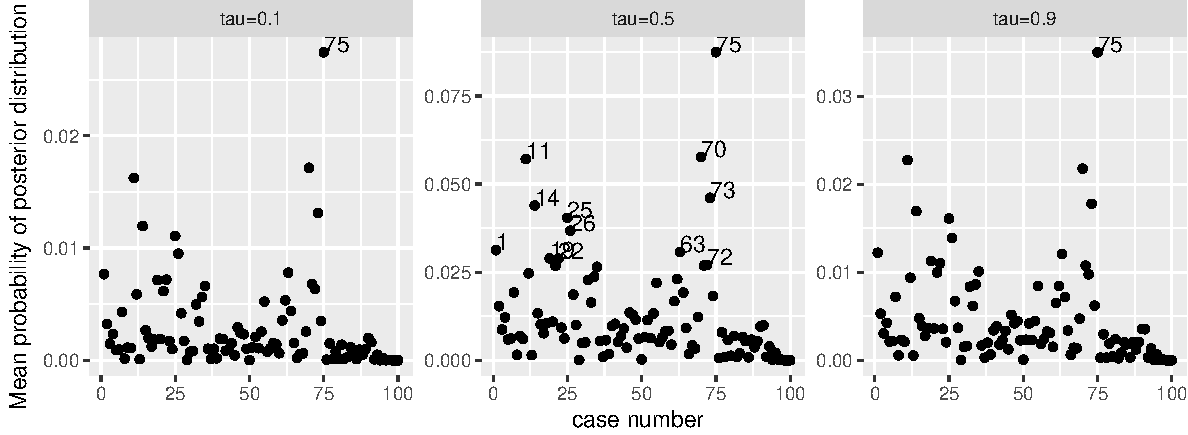
\includegraphics{Diagnosing_outliers_and_visualization_of_quantile_regression_models_files/figure-latex/unnamed-chunk-9-1} 

}

\caption{Mean posterior probability of each case on quantile 0.1, 0.5 and 0.9. The mean posterior probabilities are calculated based on the postierior distribution of latent variable using Bayesian quantile regression method}\label{fig:unnamed-chunk-9}
\end{figure}

\begin{Shaded}
\begin{Highlighting}[]
\NormalTok{kl <-}\StringTok{ }\KeywordTok{frame_bayes}\NormalTok{(y, x, tau, }\DataTypeTok{M =} \DecValTok{100}\NormalTok{,}
                  \DataTypeTok{method =} \StringTok{'bayes.kl'}\NormalTok{)}
\NormalTok{kl_m <-}\StringTok{ }\KeywordTok{cbind}\NormalTok{(case, kl)}
\KeywordTok{ggplot}\NormalTok{(kl_m, }\KeywordTok{aes}\NormalTok{(}\DataTypeTok{x =} \NormalTok{case, }\DataTypeTok{y =} \NormalTok{value)) +}
\StringTok{  }\KeywordTok{geom_point}\NormalTok{() +}
\StringTok{  }\KeywordTok{facet_wrap}\NormalTok{(~variable, }\DataTypeTok{scale =} \StringTok{'free'}\NormalTok{)+}
\StringTok{  }\KeywordTok{geom_text}\NormalTok{(}\DataTypeTok{data =} \KeywordTok{subset}\NormalTok{(kl_m, value >}\StringTok{ }\KeywordTok{mean}\NormalTok{(value) +}\StringTok{ }\DecValTok{2}\NormalTok{*}\KeywordTok{sd}\NormalTok{(value)),}
            \KeywordTok{aes}\NormalTok{(}\DataTypeTok{label =} \NormalTok{case), }\DataTypeTok{hjust =} \DecValTok{0}\NormalTok{, }\DataTypeTok{vjust =} \DecValTok{0}\NormalTok{) +}
\StringTok{  }\KeywordTok{xlab}\NormalTok{(}\StringTok{'case number'}\NormalTok{) +}
\StringTok{  }\KeywordTok{ylab}\NormalTok{(}\StringTok{'Kullback-Leibler'}\NormalTok{)}
\end{Highlighting}
\end{Shaded}

\begin{figure}

{\centering 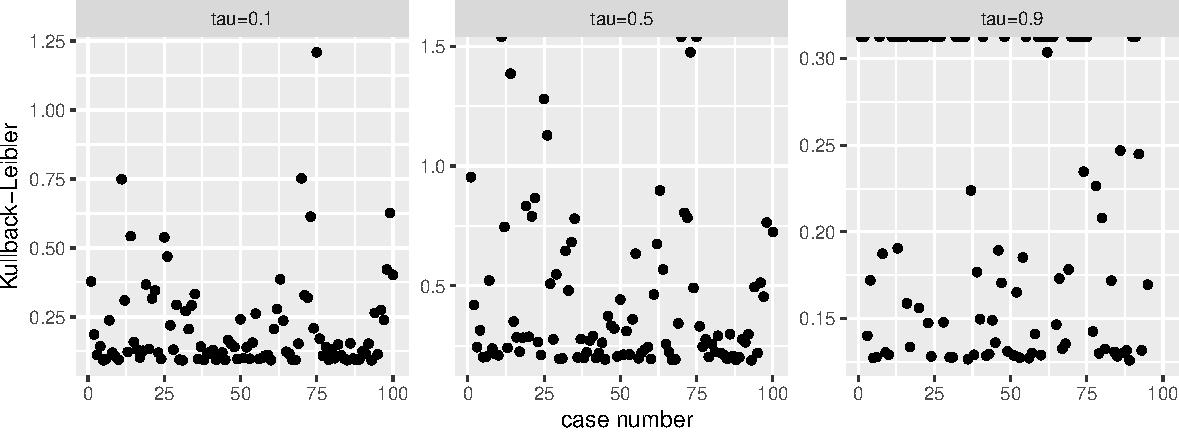
\includegraphics{Diagnosing_outliers_and_visualization_of_quantile_regression_models_files/figure-latex/unnamed-chunk-10-1} 

}

\caption{Kullback and Leibler divergence of each case on quantile 0.1, 0.5 and 0.9. The Kullback-Leibler divergence is calculated based on the postierior distribution of latent variable using Bayesian quantile regression method.}\label{fig:unnamed-chunk-10}
\end{figure}

\section{Visualizing quantile
regression}\label{visualizing-quantile-regression}

Visualization of quantile regression will help us understand the
questions `How does the shape of the model compare to the shape of the
data?'. In addition, we can have a good impression of the location of
models on each quantile. We use GGobi to visualize quantile regression
model.

\subsection{Linear quantile regression
model}\label{linear-quantile-regression-model}

In two predictors case, quantile regression models are lines in space.
We use ais data fitting models and visualize them with GGobi.

\begin{Shaded}
\begin{Highlighting}[]
\NormalTok{knitr::}\KeywordTok{include_graphics}\NormalTok{(}\KeywordTok{c}\NormalTok{(}\StringTok{"Figures/QR-model-single-pixel/linear-3D-1.png"}\NormalTok{,}
                          \StringTok{"Figures/QR-model-single-pixel/linear-3D-2.png"}\NormalTok{,}
                          \StringTok{"Figures/QR-model-single-pixel/linear-3D-3.png"}\NormalTok{,}
                          \StringTok{"Figures/QR-model-single-pixel/linear-3D-4.png"}\NormalTok{,}
                          \StringTok{"Figures/QR-model-single-pixel/linear-3D-5.png"}\NormalTok{,}
                          \StringTok{"Figures/QR-model-single-pixel/linear-3D-6.png"}\NormalTok{,}
                          \StringTok{"Figures/QR-model-single-pixel/linear-3D-7.png"}\NormalTok{,}
                          \StringTok{"Figures/QR-model-single-pixel/linear-3D-8.png"}\NormalTok{,}
                          \StringTok{"Figures/QR-model-single-pixel/linear-3D-9.png"}\NormalTok{))}
\end{Highlighting}
\end{Shaded}

\textbackslash{}begin\{center\}\includegraphics{[}width=0.2\linewidth,height=20\%{]}\{Figures/QR-model-single-pixel/linear-3D-1\}
\textbackslash{}end\{center\}

\textbackslash{}begin\{center\}\includegraphics{[}width=0.2\linewidth,height=20\%{]}\{Figures/QR-model-single-pixel/linear-3D-2\}
\textbackslash{}end\{center\}

\textbackslash{}begin\{center\}\includegraphics{[}width=0.2\linewidth,height=20\%{]}\{Figures/QR-model-single-pixel/linear-3D-3\}
\textbackslash{}end\{center\}

\textbackslash{}begin\{center\}\includegraphics{[}width=0.2\linewidth,height=20\%{]}\{Figures/QR-model-single-pixel/linear-3D-4\}
\textbackslash{}end\{center\}

\textbackslash{}begin\{center\}\includegraphics{[}width=0.2\linewidth,height=20\%{]}\{Figures/QR-model-single-pixel/linear-3D-5\}
\textbackslash{}end\{center\}

\textbackslash{}begin\{center\}\includegraphics{[}width=0.2\linewidth,height=20\%{]}\{Figures/QR-model-single-pixel/linear-3D-6\}
\textbackslash{}end\{center\}

\textbackslash{}begin\{center\}\includegraphics{[}width=0.2\linewidth,height=20\%{]}\{Figures/QR-model-single-pixel/linear-3D-7\}
\textbackslash{}end\{center\}

\textbackslash{}begin\{center\}\includegraphics{[}width=0.2\linewidth,height=20\%{]}\{Figures/QR-model-single-pixel/linear-3D-8\}
\textbackslash{}end\{center\}

\textbackslash{}begin\{center\}\includegraphics{[}width=0.2\linewidth,height=20\%{]}\{Figures/QR-model-single-pixel/linear-3D-9\}
\textbackslash{}end\{center\}

In three predictor case, quantile regression models are cuboids in space
which were displayed as follows,

\begin{Shaded}
\begin{Highlighting}[]
\NormalTok{knitr::}\KeywordTok{include_graphics}\NormalTok{(}\KeywordTok{c}\NormalTok{(}\StringTok{"Figures/QR-model-single-pixel/linear-4D-1.png"}\NormalTok{,}
                          \StringTok{"Figures/QR-model-single-pixel/linear-4D-2.png"}\NormalTok{,}
                          \StringTok{"Figures/QR-model-single-pixel/linear-4D-3.png"}\NormalTok{,}
                          \StringTok{"Figures/QR-model-single-pixel/linear-4D-4.png"}\NormalTok{,}
                          \StringTok{"Figures/QR-model-single-pixel/linear-4D-5.png"}\NormalTok{,}
                          \StringTok{"Figures/QR-model-single-pixel/linear-4D-6.png"}\NormalTok{,}
                          \StringTok{"Figures/QR-model-single-pixel/linear-4D-7.png"}\NormalTok{,}
                          \StringTok{"Figures/QR-model-single-pixel/linear-4D-8.png"}\NormalTok{,}
                          \StringTok{"Figures/QR-model-single-pixel/linear-4D-9.png"}\NormalTok{))}
\end{Highlighting}
\end{Shaded}

\textbackslash{}begin\{center\}\includegraphics{[}width=0.2\linewidth,height=20\%{]}\{Figures/QR-model-single-pixel/linear-4D-1\}
\textbackslash{}end\{center\}

\textbackslash{}begin\{center\}\includegraphics{[}width=0.2\linewidth,height=20\%{]}\{Figures/QR-model-single-pixel/linear-4D-2\}
\textbackslash{}end\{center\}

\textbackslash{}begin\{center\}\includegraphics{[}width=0.2\linewidth,height=20\%{]}\{Figures/QR-model-single-pixel/linear-4D-3\}
\textbackslash{}end\{center\}

\textbackslash{}begin\{center\}\includegraphics{[}width=0.2\linewidth,height=20\%{]}\{Figures/QR-model-single-pixel/linear-4D-4\}
\textbackslash{}end\{center\}

\textbackslash{}begin\{center\}\includegraphics{[}width=0.2\linewidth,height=20\%{]}\{Figures/QR-model-single-pixel/linear-4D-5\}
\textbackslash{}end\{center\}

\textbackslash{}begin\{center\}\includegraphics{[}width=0.2\linewidth,height=20\%{]}\{Figures/QR-model-single-pixel/linear-4D-6\}
\textbackslash{}end\{center\}

\textbackslash{}begin\{center\}\includegraphics{[}width=0.2\linewidth,height=20\%{]}\{Figures/QR-model-single-pixel/linear-4D-7\}
\textbackslash{}end\{center\}

\textbackslash{}begin\{center\}\includegraphics{[}width=0.2\linewidth,height=20\%{]}\{Figures/QR-model-single-pixel/linear-4D-8\}
\textbackslash{}end\{center\}

\textbackslash{}begin\{center\}\includegraphics{[}width=0.2\linewidth,height=20\%{]}\{Figures/QR-model-single-pixel/linear-4D-9\}
\textbackslash{}end\{center\}

\subsection{Non-linear quantile regression
model}\label{non-linear-quantile-regression-model}

In non-linear case, we use elliptic hyperboloid and hyperbolic
paraboloid as examples.

\begin{Shaded}
\begin{Highlighting}[]
\NormalTok{knitr::}\KeywordTok{include_graphics}\NormalTok{(}\KeywordTok{c}\NormalTok{(}\StringTok{"Figures/QR-model/curve1-1.png"}\NormalTok{,}
                          \StringTok{"Figures/QR-model/curve1-2.png"}\NormalTok{,}
                          \StringTok{"Figures/QR-model/curve1-3.png"}\NormalTok{,}
                          \StringTok{"Figures/QR-model/curve1-4.png"}\NormalTok{,}
                          \StringTok{"Figures/QR-model/curve1-5.png"}\NormalTok{,}
                          \StringTok{"Figures/QR-model/curve1-6.png"}\NormalTok{,}
                          \StringTok{"Figures/QR-model/curve1-7.png"}\NormalTok{,}
                          \StringTok{"Figures/QR-model/curve1-8.png"}\NormalTok{,}
                          \StringTok{"Figures/QR-model/curve1-9.png"}\NormalTok{))}
\end{Highlighting}
\end{Shaded}

\textbackslash{}begin\{center\}\includegraphics{[}width=0.2\linewidth,height=20\%{]}\{Figures/QR-model/curve1-1\}
\textbackslash{}end\{center\}

\textbackslash{}begin\{center\}\includegraphics{[}width=0.2\linewidth,height=20\%{]}\{Figures/QR-model/curve1-2\}
\textbackslash{}end\{center\}

\textbackslash{}begin\{center\}\includegraphics{[}width=0.2\linewidth,height=20\%{]}\{Figures/QR-model/curve1-3\}
\textbackslash{}end\{center\}

\textbackslash{}begin\{center\}\includegraphics{[}width=0.2\linewidth,height=20\%{]}\{Figures/QR-model/curve1-4\}
\textbackslash{}end\{center\}

\textbackslash{}begin\{center\}\includegraphics{[}width=0.2\linewidth,height=20\%{]}\{Figures/QR-model/curve1-5\}
\textbackslash{}end\{center\}

\textbackslash{}begin\{center\}\includegraphics{[}width=0.2\linewidth,height=20\%{]}\{Figures/QR-model/curve1-6\}
\textbackslash{}end\{center\}

\textbackslash{}begin\{center\}\includegraphics{[}width=0.2\linewidth,height=20\%{]}\{Figures/QR-model/curve1-7\}
\textbackslash{}end\{center\}

\textbackslash{}begin\{center\}\includegraphics{[}width=0.2\linewidth,height=20\%{]}\{Figures/QR-model/curve1-8\}
\textbackslash{}end\{center\}

\textbackslash{}begin\{center\}\includegraphics{[}width=0.2\linewidth,height=20\%{]}\{Figures/QR-model/curve1-9\}
\textbackslash{}end\{center\}

\section{Future work}\label{future-work}

high-dimensional and extreme quantile work.

\section{Reference}\label{reference}

Koenker R, Machado J A F. Goodness of fit and related inference
processes for quantile regression{[}J{]}. Journal of the american
statistical association, 1999, 94(448): 1296-1310.

Fitzenberger B. The moving blocks bootstrap and robust inference for
linear least squares and quantile regressions{[}J{]}. Journal of
Econometrics, 1998, 82(2): 235-287.

Chernozhukov V, Hansen C. Instrumental variable quantile regression: A
robust inference approach{[}J{]}. Journal of Econometrics, 2008, 142(1):
379-398.

Geraci M, Bottai M. Quantile regression for longitudinal data using the
asymmetric Laplace distribution{[}J{]}. Biostatistics, 2007, 8(1):
140-154.

Koenker R. Quantile regression for longitudinal data{[}J{]}. Journal of
Multivariate Analysis, 2004, 91(1): 74-89.

Korobilis D. Quantile regression forecasts of inflation under model
uncertainty{[}J{]}. International Journal of Forecasting, 2017, 33(1):
11-20.

Autor D H, Houseman S N, Kerr S P. The Effect of Work First Job
Placements on the Distribution of Earnings: An Instrumental Variable
Quantile Regression Approach{[}J{]}. Journal of Labor Economics, 2017,
35(1): 149-190.

Mitchell J A, Dowda M, Pate R R, et al. Physical Activity and Pediatric
Obesity: A Quantile Regression Analysis{[}J{]}. Medicine and science in
sports and exercise, 2017, 49(3): 466.

Gallego-Álvarez I, Ortas E. Corporate environmental sustainability
reporting in the context of national cultures: A quantile regression
approach{[}J{]}. International Business Review, 2017, 26(2): 337-353.

Maciejowska K, Nowotarski J, Weron R. Probabilistic forecasting of
electricity spot prices using Factor Quantile Regression
Averaging{[}J{]}. International Journal of Forecasting, 2016, 32(3):
957-965.

Parente P M D C, Santos Silva J. Quantile regression with clustered
data{[}J{]}. Journal of Econometric Methods, 2016, 5(1): 1-15.

Galvao A F, Kato K. Smoothed quantile regression for panel data{[}J{]}.
Journal of Econometrics, 2016, 193(1): 92-112.

Arellano M, Bonhomme S. Nonlinear panel data estimation via quantile
regressions{[}J{]}. The Econometrics Journal, 2016, 19(3).

Canay I A. A simple approach to quantile regression for panel
data{[}J{]}. The Econometrics Journal, 2011, 14(3): 368-386.

Geraci M. Linear quantile mixed models: the lqmm package for Laplace
quantile regression{[}J{]}. Journal of Statistical Software, 2014,
57(13): 1-29.

Chernozhukov V, Hansen C. Instrumental quantile regression inference for
structural and treatment effect models{[}J{]}. Journal of Econometrics,
2006, 132(2): 491-525.


\end{document}
